\documentclass[
10pt,					% Schriftgröße
a4paper,				% A4 paper
twoside,				% Zweiseitig
BCOR=8mm,				% Bindekorrektur inkl. Biegefalz
headings=normal,		% Kleinere Kapitelüberschriften => check preamble
headsepline,			% Enable line to seperate head ...
footsepline,			% ... and foot
plainfootsepline,		% Footseperation line on chapter start
%,draft
]{scrbook}

\usepackage[
top=30mm,
bottom=55mm,
inner=25mm,
outer=30mm,
%marginparsep=7mm,
%marginparwidth=48mm,
%paperwidth=210mm,
%paperheight=245mm, 286mm (A4)
]{geometry}

\usepackage[utf8]{inputenc}
% when latex complains about unicode char U+2212 is not configured for use in latex use the line below
\DeclareUnicodeCharacter{2212}{-}% support older LaTeX versions
%\usepackage[latin1]{inputenc}
\usepackage[T1]{fontenc}
\usepackage{lmodern}
\usepackage[english]{babel}
\usepackage{csquotes}
\usepackage{amsmath}
\usepackage{textcomp}		%enables \textdegree to use as �
\usepackage{amsfonts}
\usepackage{amssymb}
\usepackage{graphicx}
\usepackage{xhfill}			% provides /hrulefill (disclaimer)
%\usepackage{wasysym}		
\usepackage{braket}		% fur <A|H|B> <A| |A> oder <A>
%\DeclareGraphicsExtensions{.pdf,.png,.jpg}
%%%%%%%%%%%%%%%%%%%%%%%%%%%%%
\usepackage{siunitx}
\DeclareSIUnit\langmuir{L}
%%%%%%%%%%%%%%%%%%%%%%%%%%%%%
\usepackage[hidelinks,breaklinks=true]{hyperref}
%\usepackage{url}
\usepackage[section]{placeins} %definiert \floatbarrier, mit option automatisch bei jeder section
%%%%%%%%%%%%%%%%%%%%%%%%%%%%%%%%%%%%%%%%%%%
\usepackage{subfigure}
\usepackage{wrapfig}
%%%%%%%%%%%%%%%%%%%%%%%%%%%%%%%%%%%%%%%%%%%
\usepackage{caption}
\usepackage{microtype}
%\usepackage{subcaption}
\usepackage{multicol}
\usepackage{multirow}
%%%%%%%%%%%%%%%%%%%%%%%%%%%%
% fuer Stichwortverzeichnis
\usepackage{makeidx}
% Stichwortverzeichnis erstellen
\makeindex
%%%%%%%%%%%%%%%%%%%%%%%%%%%%%%%%%%%%%%%%%%%%%%%%%%%%%%%
\usepackage[style=numeric		% bibliogryphy-styles: alphabetic, numeric, chem-angew, ieee, nature, science
,backend=biber
%,refsection=chapter			% setzt bibliographies nach chaptern getrennt, nach jedem chapter muss ein 
								% printbibliogrphy stehen
]{biblatex} 	
\addbibresource{./bib.bib}  	% relative to root directory (where the file that includes this file is located)! 
								%do NOT OMIT .bib ending

%avoids ugly line breaks within bibligraphy
\addto\bibsetup{\setlength{\emergencystretch}{1.5em}} 	

% Zum Verwalten der Zitate benutze ich Zotero, zum Erzeugen der .bib-Datein f�r Latex wird die Exportfunktion von Zotero benutzt (rechtsklick auf ``Meine Bibliothek'' im linken Reiter: Option Biblatex in die Datei bib-zotero-export.bib aus welcher ich dann die betreffenden Zitate auf Richtigkeit \"uberpr\"ufe und in die bib.bib kopiere.
%%%%%%%%%%%%%%%%%%%%%%%%%%%%%%%%%%%%%%%%%%%%%%%%%%%%%%%
% \usepackage[top=2.5cm,left=2.5cm,right=3.5cm,bottom=3.5cm]{geometry}
%%%%%%%%%%%%%%%%%%%%%%%%%%%%%%%%%%%%%%%%%%%%%%%%%%%%%%%
\usepackage{xcolor}
%%%%%%%%%%%%%%%%%%%%%%%%%%%%%%%%%%%%%%%%%%%%%%%%%%%%%%
%%%%%%%%%%%%%%%%%%%%%%%%%%%%%%%%%%%%%%%%%%%%%%%%%%%%%%
\usepackage[draft=false]{scrlayer-scrpage}		%deaktiviert ruler in der draft version
\pagestyle{scrheadings}
%%%%%%%%%%%%%%%%%%%%%%%%%%%%%%%%%%%%%%%%%%%%%%%%%%%%%%
%%%%%%%%%%%%%%%%% DAUMENKINO Footer %%%%%%%%%%%%%%%%%%
	\usepackage{etex}
	\usepackage{intcalc} 
	\newcommand*{\AnzBilder}{200}		            		%<--Variablen anpassen
\newcommand*{\KinoPfad}{./images/animation/lumo/} 	%<--Variablen anpassen

%%%%Quelltext%%%
\newcommand*{\SafeboxName}{sbKino}

\makeatletter
%Erzeugt neue Saveboxen und füllt sie mit includegraphics-Anweisungen
%Aufruf: \NewSaveBoxes{sbKino}{5}{daumenkino/kino}
\newcommand*{\NewSaveBoxes}[3]{%
	\@tempcnta 1
	\@whilenum \@tempcnta< \numexpr(#2+1) \do{%
		%Savebox anlegen
		\expandafter\newsavebox\csname #1\the\@tempcnta\endcsname
		%Savebox mit Leben füllen
		\expandafter\savebox\csname #1\the\@tempcnta\endcsname{%
			\includegraphics[width=0.5cm]{#3\the\@tempcnta}%
		}%
		\advance\@tempcnta 1
	}%
}

\newcommand*{\bildnr}{\numexpr\intcalcMod{\numexpr\value{page}}{\numexpr\AnzBilder}\relax}
\newcommand*{\lumoseries}{%
	\usebox{\@nameuse{\SafeboxName\the\bildnr}}%
}
\makeatother
\NewSaveBoxes{\SafeboxName}{\AnzBilder}{\KinoPfad}
	%inner side of odd pages
	\lofoot[\lumoseries]{\lumoseries} % Add flicker books to [plain.scrheadins] and {scrheadins}!
	% inner side of even pages	
	\newcommand*{\AnzBilderLogo}{200}		            		%<--Variablen anpassen
\newcommand*{\KinoPfadLogo}{./images/animation/logo/} 	%<--Variablen anpassen
%%%%Quelltext%%%
\newcommand*{\SafeboxNameLogo}{sbKinologo}

\makeatletter
%Erzeugt neue Saveboxen und füllt sie mit includegraphics-Anweisungen
%Aufruf: \NewSaveBoxesLogo{sbKino}{5}{daumenkino/kino}
\newcommand*{\NewSaveBoxesLogo}[3]{%
	\@tempcntb 1
	\@whilenum \@tempcntb< \numexpr(#2+1) \do{%
		%Savebox anlegen
		\expandafter\newsavebox\csname #1\the\@tempcntb\endcsname
		%Savebox mit Leben füllen
		\expandafter\savebox\csname #1\the\@tempcntb\endcsname{%
			\includegraphics[width=0.5cm]{#3\the\@tempcntb}%
		}%
		\advance\@tempcntb 1
	}%
}
%intcalc-version
\newcommand*{\bildnrLogo}{\numexpr\intcalcMod{\numexpr\value{page}}{\numexpr\AnzBilderLogo}\relax}

\newcommand*{\logoseries}{%
	\usebox{\@nameuse{\SafeboxNameLogo\the\bildnrLogo}}%
}
\makeatother
\NewSaveBoxesLogo{\SafeboxNameLogo}{\AnzBilderLogo}{\KinoPfadLogo}
%%%Aufruf%%%%%%%
	\refoot[\logoseries]{\logoseries} % Add flicker books to [plain.scrheadins] and {scrheadins}!
%%%%%%%%%%%%%%%%%%%%%%%%%%%%%%%%%%%%%%%%%%%%%%%%%%%%%%
%%%%%%%%%%%%%%%%%%%%%%%%%%%%%%%%%%%%%%%%%%%%%%%%%%%%%%
% Basic information for cover & title page
\newcommand*{\getUniversity}{Technische Universit\"at M\"unchen}
\newcommand*{\getFaculty}{Department of physics}
\newcommand*{\getFacultyger}{Fakult\"at f\"ur Physik}
\newcommand*{\getTitle}{Molecular adsorption on \textit{h}-BN}
%newcommand*{\getTitleger}{TODO: Titel der Abschlussarbeit}
\newcommand*{\getAuthor}{Domenik Matthias Zimmermann}
\newcommand*{\getDoctype}{Dissertation}
\newcommand*{\getDoctypeger}{Vollst\"andiger Abdruck der von der Fakult\"at für Physik der Technischen Universit\"at M\"unchen zur Erlangung des akademischen Grades eines Doktors der Naturwissenschaften (Dr. rer. nat.) genehmigten Dissertation.}
\newcommand*{\getSupervisor}{Prof.\ Dr.\ Wilhelm Auw\"arter}
\newcommand*{\getChairman}{TODO: Chairman}
\newcommand*{\getFirstExaminer}{TODO: 1. Examiner}
\newcommand*{\getSecondExaminer}{TODO: 2. Examiner}
\newcommand*{\getSubmissionDate}{TODO: Submission date}
\newcommand*{\getSubmissionLocation}{Munich}
\newcommand*{\getDisclaimer}{I assure the single handed composition of this \MakeLowercase{\getDoctype{}} only supported by declared resources.}
% TODO: add custom commands etc.

%%%%%%%%%%%%%%%%%%%%%%%%%%%%%%%%%%%%%%%%%%%%%%%%%%%%%%%%%%%%%%%%%%%%%%%%%%%%%%%%%%%%%%%%%%%%%
% Change \autoref (Figure x.x) to FIGURE x.x

%%%%%%%%%%%%%%%%%%%%%%%%%%%%%%%%%%%%%%%%%%%%%%%%%%%%%%%%%%%%%%%%%%%%%%%%%%%%%%%%%%%%%%%%%%%%%
% Python style for highlighting
% Check https://tex.stackexchange.com/questions/83882/how-to-highlight-python-syntax-in-latex-listings-lstinputlistings-command#83883

% Default fixed font does not support bold face
\DeclareFixedFont{\ttb}{T1}{txtt}{bx}{n}{12} % for bold
\DeclareFixedFont{\ttm}{T1}{txtt}{m}{n}{12}  % for normal

\newcommand\pythonstyle{\lstset{
		language=Python,
		basicstyle=\small,             %\ttm, \tiny \small
		otherkeywords={self},             % Add keywords here
		keywordstyle=\small\color{deepblue},
		emph={MyClass,__init__},          % Custom highlighting
		emphstyle=\small\color{deepred},    % Custom highlighting style
		stringstyle=\color{deepgreen},
		frame=tb,                         % Any extra options here
		showstringspaces=false,           % 
		frame=single,
		numbers = left,
		numbersep=5pt
}}
% Python environment
\lstnewenvironment{python}[1][]
{
	\pythonstyle
	\lstset{#1}
}
{}
% Python for external files
\newcommand\pythonexternal[2][]{{
		\pythonstyle
		\lstinputlisting[#1]{#2}}}
% Python for inline
\newcommand\pythoninline[1]{{\pythonstyle\lstinline!#1!}}
%%%%%%%%%%%%%%%%%%%%%%%%%%%%%%%%%%%%%%%%%%%%%%%%%%%%%%%%%%%%%%%%%%%%%%%%%%%%%%%%%%%%%%%%%%%%%


\begin{document}
\section{asd}
The tunneling effect describes the behavior of a particle that faces a potential barrier. In the classical picture the particle is prohibited to move across the potential barrier if its energy is lower than the barrier height. In quantum mechanics however, the particle is described as wave. When this now faces the potential barrier, a fraction of the wave package transmitted through the barrier - an effect known as tunneling.

\subsection{An historic overview}
The tunneling effect was first observed by Hund in 1926 in molecules, where he explained the sharing of an electron between atoms, each separated by a potential well.\cite{Mehra_tunneling_1982} A principle fundamental for an understanding of covalent chemical bonds. 

The first quantitative expression of the tunneling current between two vacuum serperated metals was introduced by Bardeen in 1961.\cite{Bardeen_tunneling_1961} 

This lead to an early experiment build by Russell Young, John Ward and Fredric Scire in 1972.\cite{Young_topographiner_1972} Here the basic principles are shown already (tunneling with metal tip). The concept was further improved by Binning \& Rohrer in 1981 \cite{binning_tunneling_1982} when they were the first to report experimental evidence for the tunneling through an vacuum gap. Its width was controlled with ceramics exhibiting the piezoelectric effect. They showcased the excelled resolution capabilities by resolving the ($7 \times 7$) reconstruction of the Si(111) surface \cite{binnig_1983} and received the noble prize in 1986 for "their design of the scanning tunneling microscope" (STM).\cite{_noble_price_1986} 

In the following the tunneling process through a vacuum gap between metallic tip and sample will be summarized addressed theoretically and used as model system to describe the basic concept of STM.

\subsection{Basic principles}
\index{STM!One dimensional tunneling}

\begin{figure}[]\centering
	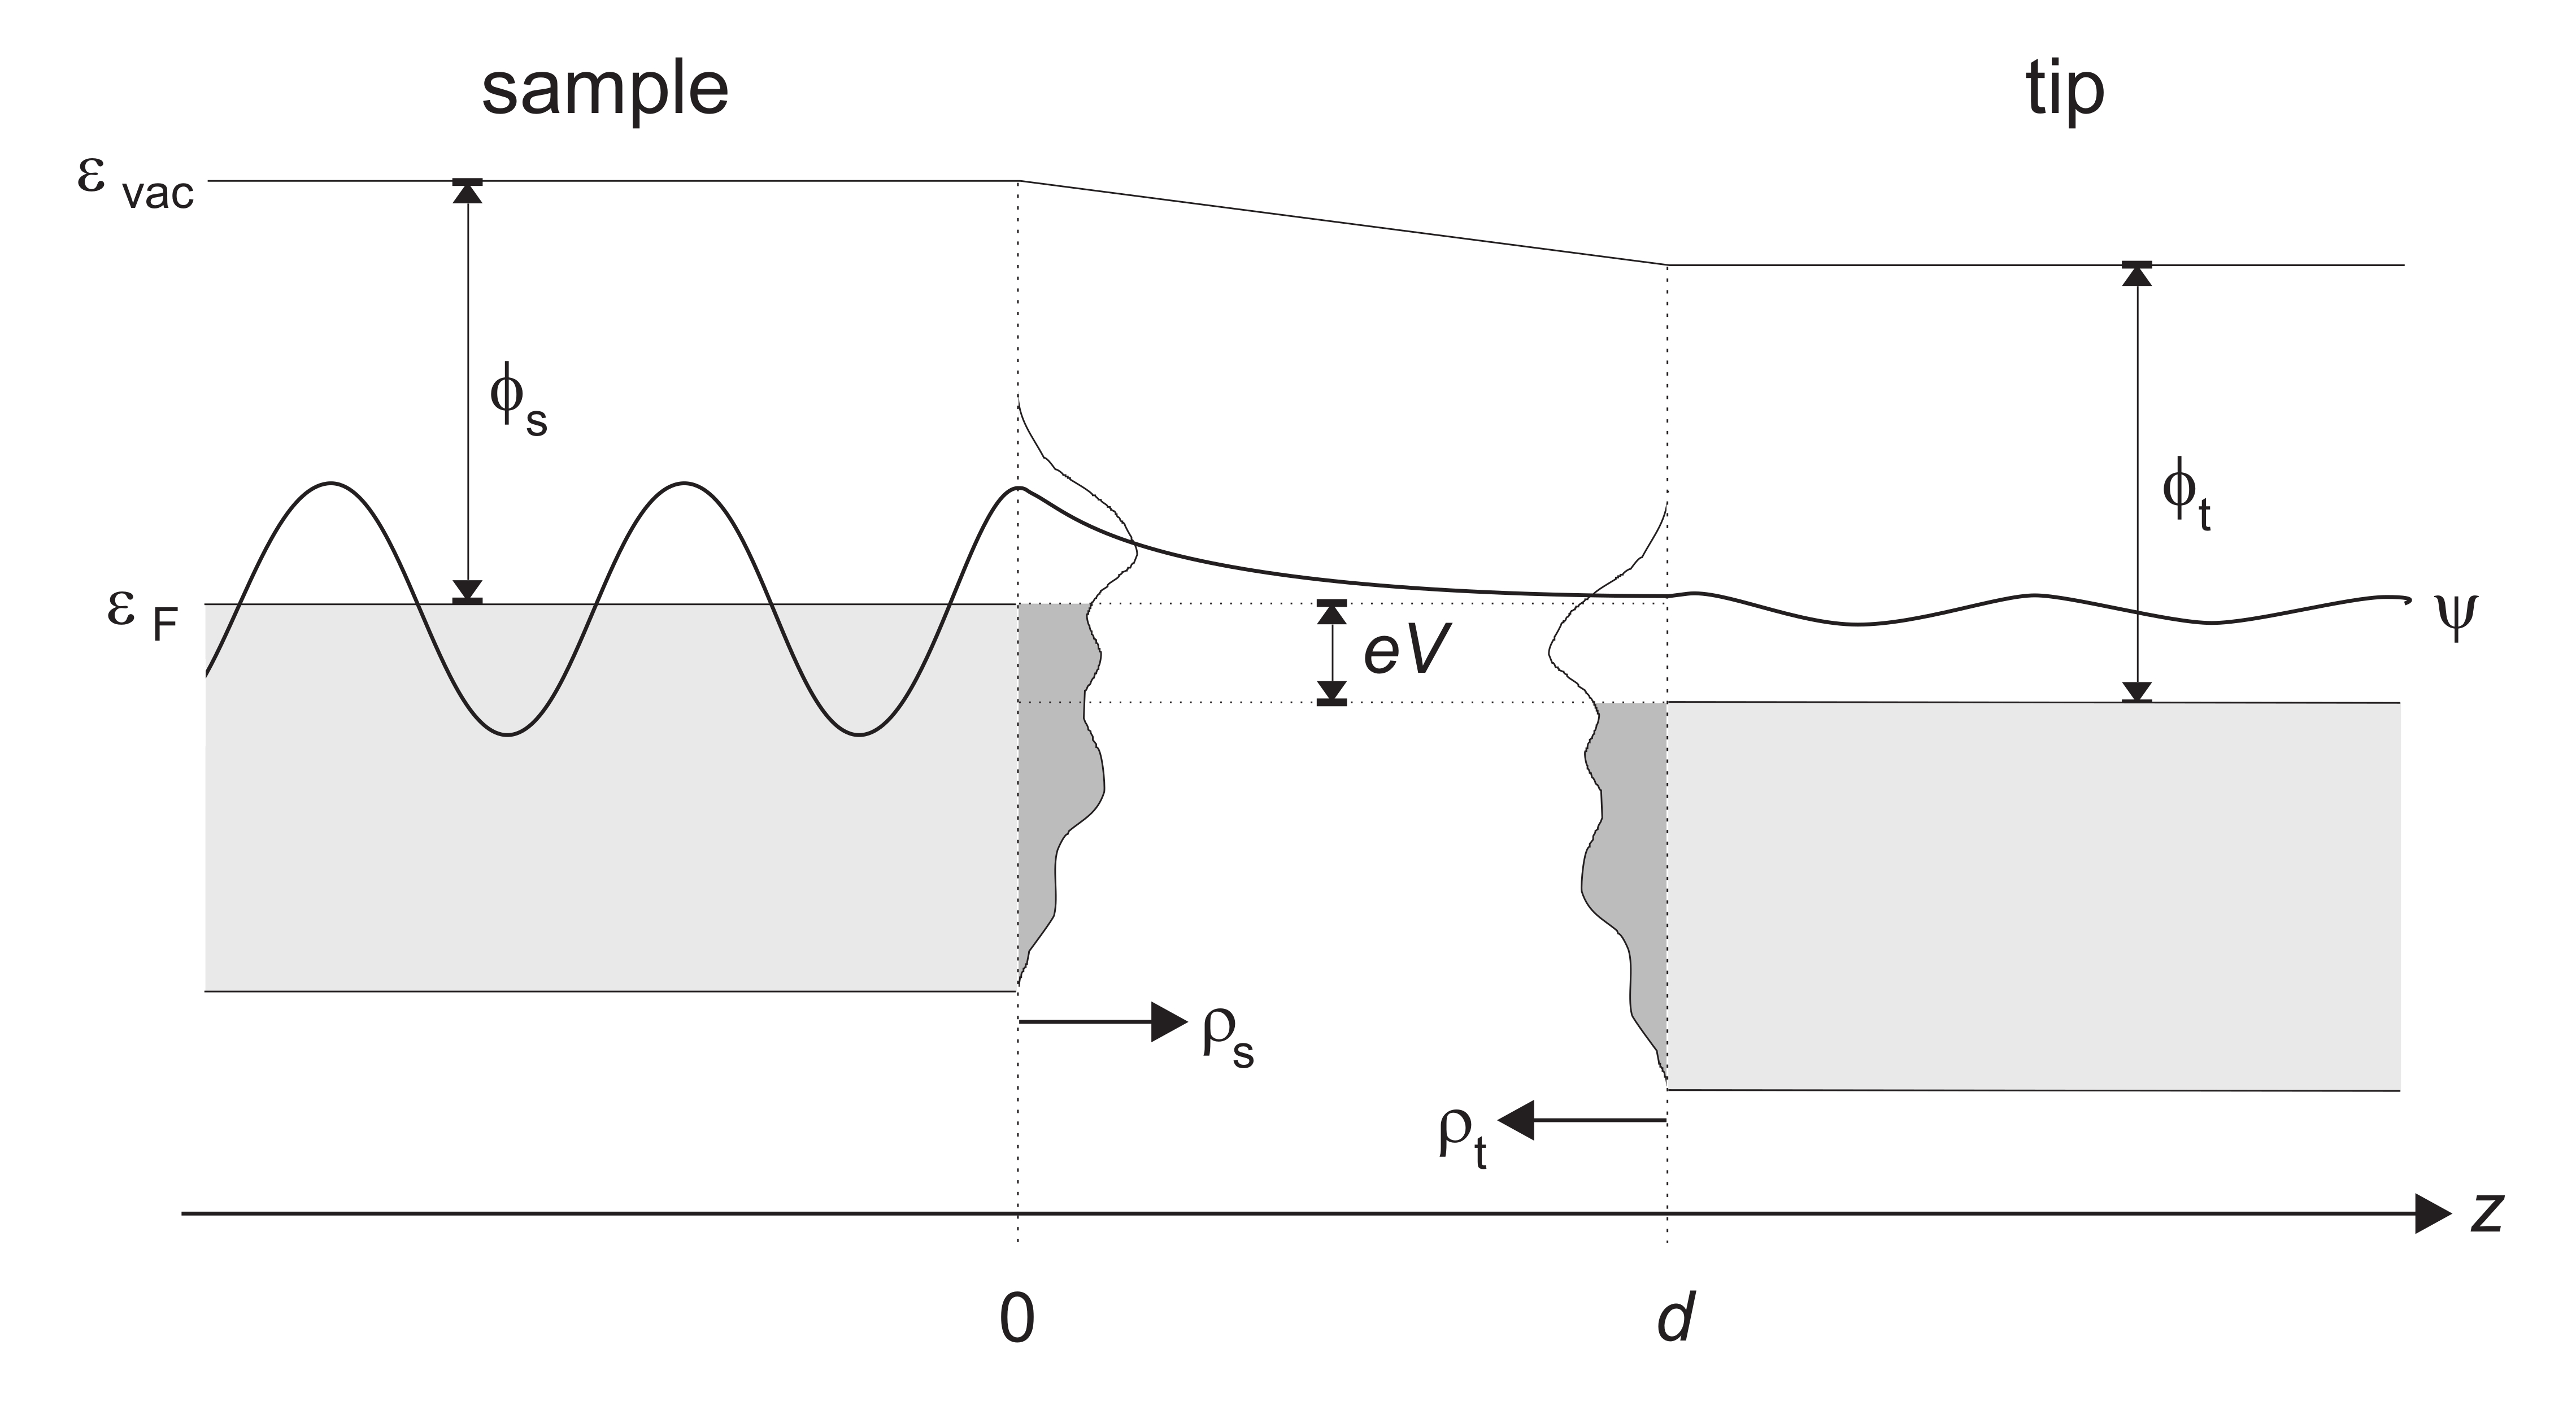
\includegraphics[width=0.7\textwidth]{./images/tunnel-barrier}
	\caption{Energy diagram to visualize the tunneling process between sample (left) and tip (right) separated by a distance d. Work functions of sample and tip ($\Phi_s$ and $\Phi_t$) separate the filled states (shaded regions) and the vacuum level ($\epsilon_{vac}$). Since sample ($\rho_s$) and tip DOS ($\rho_t$) may not be uniform, a fictional DOS is sketched in darker colors between both. The samples energy is lifted by $eV$ after a bias is applied and results in a net electron current from the sample into the tip. One tunneling process is indicated by a wave function in the sample. After overcoming the vacuum barrier its amplitude decreased and the corresponding electron occupies a free state (white) in the tip material.  Adopted from \cite{diss-schunack}}
	\label{fig:STM-barrier}
\end{figure}

Consider a system where two metals (sample and tip) are separated by a vacuum gap. 

The amount of energy needed to remove an electron from the metals highest occupied energy level ($E_F$, Fermi energy) is called work function $\Phi$. It depends on the electrostatic potential $\phi_E$ that has to be overcome by an electron charge $e$ at the surface.
$$ \Phi = -e \phi_E - E_F $$

\autoref{fig:STM-barrier} shows an energy diagram for tip and sample. The work function $\Phi_s$ (sample) and $\Phi_t$ (tip) separates the vacuum level $\epsilon_{vac}$ and Fermi energy $E_F$

If sample and tip are in thermodynamic equilibrium, their Fermi energies are equal.
When both are brought in close contact, electrons from the sample tunnel into unoccupied states of the tip and vice versa in the same number. Hereby electrons close to $E_F$ have the largest decay length and attenuate less strong in vacuum and contribute strongest to the tunneling current.

The samples potential can be changed by applying a voltage $V=U_b$ to it. This lifts its Fermi energy with respect to the tips and leads to  a net electron current from the sample into the tip. Reversing the voltage results in electrons tunneling from the tip into the sample. The current can be modeled and calculated in simple systems. 

In the model of model of Tersoff-Hamann\index{STM!Tersoff-Hamann} the tip is atomically sharp and its electrons waveform is s-like. Further assuming low temperature and a constant band structure for the tip, it is possible to calculate 
the tunneling current $I$. It is for an s-wave like tip with radius R. 

$$I \propto U \rho_t(E_F)\rho_s(E_F)R^2\kappa^{-4}e^{2\kappa R} $$

With this theory constant current STM images image the surface density of states for  a given voltage $U$. The exponential decay of an electron wave function into vacuum limits ($\propto e^-\kappa d$) the current, which is proportional to the squared amplitude of it. $$I\propto e^{-2\kappa d}$$
Like in one dimension the current depends on the barrier height ($\kappa=\frac{\sqrt{2m\Phi}}{\hbar}$). Increasing the distance exponentially decreases the tunneling current.
% $$I=32\pi^3\hbar^{-1}e^2V\Phi_t^2 R^2\kappa^{-4}e^{-2\kappa R}\rho_t(E_F)\rho_s(r_o,E_F)$$ Here the current is described in relation to $\rho_t$ the density of states per unit volume of the tip, R the tip radius and $\rho_s(r_0,E_F)$ the Fermi level density of states in the sample\cite{bonnell_scanning_1993}. The distance between tip and sample is denoted as \textcolor{red}{\textbf{$Z$}} and the inverse decay length of the electrons wave function is $\kappa=\frac{\sqrt{2m\Phi_t}}{\hbar}$. 

%While the tip is far away from the sample, its vacuum levels is the same. The corresponding Fermi energies of sample and tip lie below the vacuum level by the amount of their work functions ($\Phi_s$ and $\Phi_t$ for sample and tip respectively). 

%Wave functions of electrons within the tip and sample decay exponentially in vacuum, depended on their energy with respect to the Fermi level.

% Electrons now face a potential barrier (approximately rectangular) which can be overcome if their energy is high enough and the barrier sufficiently narrow. When a voltage is applied across the tunneling barrier, the energy of the tip-electrons is shifted by $eV$ as illustrated in \autoref{fig:STM-barrier}. When a positive bias voltage is applied, electrons tunnel from the tip into unoccupied states in the sample - a negative bias results in a tunneling current in opposite direction. 
%
%Following the 
%Tersoff-Hamann\footnote{Please's note that there are more models and corrections to them. An evolution from Bardeen's approach to the one done by Tersoff-Hamann can be found here \cite{lounis_theory_2014, wortmann_interpretation_2000} including Chen's expansion.}((1) uniform density of states in the tip, (2) temperature is low, (3) small bias voltage of some mV, (4) waveform of electrons in tip are s-waves) the tunneling current measured at the center of the curvature of the s-wave like tip results to $$I=32\pi^3\hbar^{-1}e^2V\Phi_t^2 R^2\kappa^{-4}e^{-2\kappa R}\rho_t(E_F)\rho_s(r_o,E_F)$$ Here the current is described in relation to $\rho_t$ the density of states per unit volume of the tip, R the tip radius and $\rho_s(r_0,E_F)$ the Fermi level density of states in the sample\cite{bonnell_scanning_1993}. The distance between tip and sample is denoted as \textcolor{red}{\textbf{$Z$}} and the inverse decay length of the electrons wave function is $\kappa=\frac{\sqrt{2m\Phi_t}}{\hbar}$. 
If $I$ is held constant one can see that the tip in principle follows a contour of constant Fermi level density of states at the sample surface. While its a good first approximation of the system, in many cases the bias is in the range of (\SIrange{1}{5}{\V}) so more than just the electrons near Fermi contribute. Also a uniform $\rho_t$ may not be accurate in all cases.

Using \index{STM!WKB} Wentzel-Kramers-Brillouin (WKB) theory\cite{wentzel_verallgemeinerung_1926, kramers_wellenmechanik_1926, brillouin_mecanique_1926} the tunneling current is given by
\begin{equation}
I=\int_0^{eV}\rho_s(r,E)\rho_t(r,eV+E)T(E,eV,r)dE
\label{WKB}
\end{equation}
where $\rho_s(\rho_t)$ is the density of states of the sample (tip) and T is the tunneling transmission probability
\begin{equation}
T(E,eV)=exp\left(-\frac{\textcolor{red}{\textbf{2}}Z\sqrt{2m}}{\hbar}\sqrt{\frac{\Phi_s+\Phi_t}{2}+\frac{eV}{2}-E}\right)
\label{Transmission-function} 
\end{equation}
describing the propability of an tunneling event between tip and sample.

If $eV<0$ the tunneling current is largest for $E=0$ (electrons on the Fermi-level of the sample), if $eV>0$ the tunneling current is largest for $E=eV$ (electrons of Fermi level in tip).

Since states with highest energy have the largest decay lengths in vacuum, most of the tunneling current is determined by electrons within close proximity to the Fermi level.\footnote{More information related to tunneling processes can be found here \cite{bonnell_scanning_1993}.}

Due to the fact that the tunneling current is proportional the density of states in the tip and the molecule one can deduce the band structure within a range of several volts in the vicinity of the Fermi energy.

Investigation of this behavior led to the establishment of a new measurement technique, called scanning tunneling spectroscopy (see \autoref{section:STS}). 

\end{document}